
%{{第十二回}}{第十二回}}

\chapter{王熙凤毒设相思局\hspace{.5em}贾天祥正照风月鉴}

{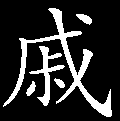
\includegraphics[width=3mm]{../Images/00005}  \kaishu  反正从来总一心,镜光至意两相寻。有朝敲破蒙头瓮,绿水青山任好春。}

话说凤姐正与平儿说话,只见有人回说:``瑞大爷来了。''凤姐急命:{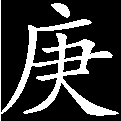
\includegraphics[width=3mm]{../Images/00004}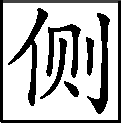
\includegraphics[width=3mm]{../Images/00011}\footnotesize \kaishu 立意追命。}``快请进来。''贾瑞见往里让,心中喜出望外,急忙进来,见了凤姐,满面陪笑,{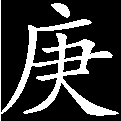
\includegraphics[width=3mm]{../Images/00004}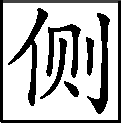
\includegraphics[width=3mm]{../Images/00011}\footnotesize \kaishu 如蛇。}连连问好。凤姐儿也假意殷勤,让坐让茶。

贾瑞见凤姐如此打扮,益发酥倒,因饧了眼问道:``二哥哥怎么还不回来?''凤姐道:``不知什么原故。''贾瑞笑道:``别是路上有人绊住了脚了,{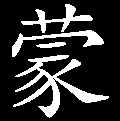
\includegraphics[width=3mm]{../Images/00006}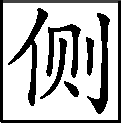
\includegraphics[width=3mm]{../Images/00011}\footnotesize \kaishu 旁敲远引。}舍不得回来也未可知?''凤姐道:``也未可知。男人家见一个爱一个也是有的。''{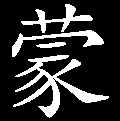
\includegraphics[width=3mm]{../Images/00006}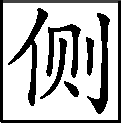
\includegraphics[width=3mm]{../Images/00011}\footnotesize \kaishu 这是钩。}贾瑞笑道:{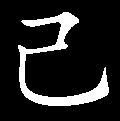
\includegraphics[width=3mm]{../Images/00003}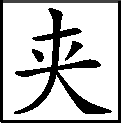
\includegraphics[width=3mm]{../Images/00012}\footnotesize \kaishu 如闻其声。}``嫂子这话错了,我就不这样。''{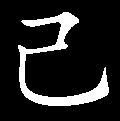
\includegraphics[width=3mm]{../Images/00003}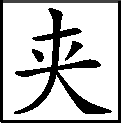
\includegraphics[width=3mm]{../Images/00012}\footnotesize \kaishu 渐渐入港。}凤姐笑道:``像你这样的人能有几个呢,十个里也挑不出一个来。''{{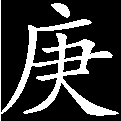
\includegraphics[width=3mm]{../Images/00004}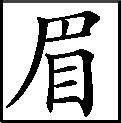
\includegraphics[width=3mm]{../Images/00010}\footnotesize \kaishu 勿作正面看为幸。畸笏。 }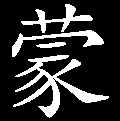
\includegraphics[width=3mm]{../Images/00006}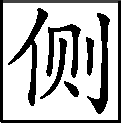
\includegraphics[width=3mm]{../Images/00011}\footnotesize \kaishu 游鱼虽有入釜之志,无钩不能上岸;一上钩来,欲去亦不可得。}贾瑞听了,喜的抓耳挠腮,又道:``嫂子天天也闷的很?''凤姐道:``正是呢,只盼个人来说话解解闷儿。''贾瑞笑道:``我倒天天闲着,天天过来替嫂子解解闲闷可好不好?''凤姐笑道:``你哄我呢,你那里肯往我这里来?''贾瑞道:``我在嫂子跟前,若有一点谎话,天打雷劈!只因素日闻得人说,嫂子是个利害人,在你跟前一点也错不得,所以唬住了我。如今见嫂子最是个有说有笑极疼人的,{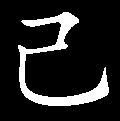
\includegraphics[width=3mm]{../Images/00003}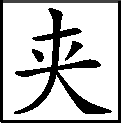
\includegraphics[width=3mm]{../Images/00012}\footnotesize \kaishu 奇妙!}我怎么不来,------死了也愿意!''{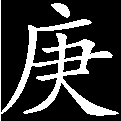
\includegraphics[width=3mm]{../Images/00004}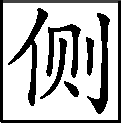
\includegraphics[width=3mm]{../Images/00011}\footnotesize \kaishu 这倒不假。}凤姐笑道:``果然你是个明白人,比贾蓉两个强远了。我看他那样清秀,只当他们心里明白,谁知竟是两个糊涂虫,{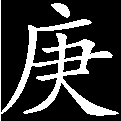
\includegraphics[width=3mm]{../Images/00004}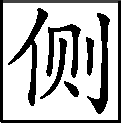
\includegraphics[width=3mm]{../Images/00011}\footnotesize \kaishu 反文,着眼。}一点不知人心。''

贾瑞听这话,越发撞在心坎儿上,由不得又往前凑了一凑,{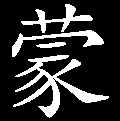
\includegraphics[width=3mm]{../Images/00006}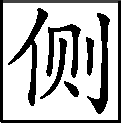
\includegraphics[width=3mm]{../Images/00011}\footnotesize \kaishu 写呆人痴性活现。}觑着眼看凤姐带的荷包,然后又问戴着什么戒指。凤姐悄悄道:``放尊重着,别叫丫头们看了笑话。''贾瑞如听纶音佛语一般,忙往后退。凤姐笑道:``你该去了。''{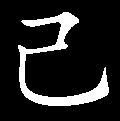
\includegraphics[width=3mm]{../Images/00003}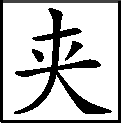
\includegraphics[width=3mm]{../Images/00012}\footnotesize \kaishu 叫``去'',正是叫``来''也。}贾瑞道:``我再坐一坐儿。好狠心的嫂子!''凤姐又悄悄的道:``大天白日,人来人往,你就在这里也不方便。你且去,等着晚上起了更你来,悄悄的在西边穿堂儿等我。''{{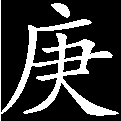
\includegraphics[width=3mm]{../Images/00004}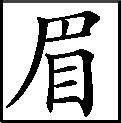
\includegraphics[width=3mm]{../Images/00010}\footnotesize \kaishu 先写穿堂,只知房舍之大,岂料有许多用处。 }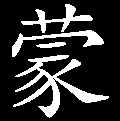
\includegraphics[width=3mm]{../Images/00006}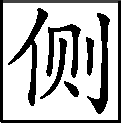
\includegraphics[width=3mm]{../Images/00011}\footnotesize \kaishu 凡人在平静时,物来言至,无不照见。若迷于一事一物,虽风雷交作,有所不闻。即``穿堂儿等''之一语,府第非比凡常,关启门户,必要查看,且更夫仆妇,势必往来,岂容人藏过于其间?只因色迷,闻声连诺,不能有回思之暇,信可悲夫!}贾瑞听了,如得珍宝,忙问道:``你别哄我。但只那里人过的多,怎么好躲的?''凤姐道:``你只放心。我把上夜的小厮们都放了假,两边门一关,再没别人了。''贾瑞听了,喜之不尽,忙忙的告辞而去,心内以为得手。{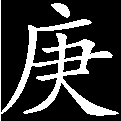
\includegraphics[width=3mm]{../Images/00004}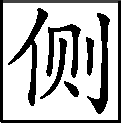
\includegraphics[width=3mm]{../Images/00011}\footnotesize \kaishu 未必。}

盼到晚上,果然黑地里摸入荣府,趁掩门时,钻入穿堂。果见漆黑无人,往贾母那边去的门户已锁,倒只有向东的门未关。贾瑞侧耳听着,半日不见人来,忽听``咯登''一声,东边的门也倒关了。{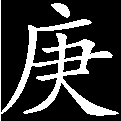
\includegraphics[width=3mm]{../Images/00004}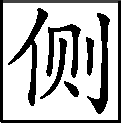
\includegraphics[width=3mm]{../Images/00011}\footnotesize \kaishu 平平略施小计。}贾瑞急的也不敢则声,只得悄悄的出来,将门撼了撼,关得铁桶一般。此时要求出去,亦不能够。{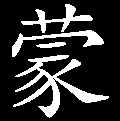
\includegraphics[width=3mm]{../Images/00006}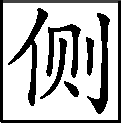
\includegraphics[width=3mm]{../Images/00011}\footnotesize \kaishu 此大抵是凤姐调遣。不先为点明者,可以少许多事故,又可以藏拙。}南北皆是大房墙,要跳亦无攀援。这屋内又是过门风,空落落;现是腊月天气,夜又长,朔风凛凛,侵肌裂骨,一夜几乎不曾冻死。{{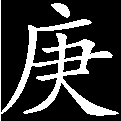
\includegraphics[width=3mm]{../Images/00004}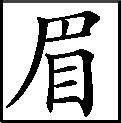
\includegraphics[width=3mm]{../Images/00010}\footnotesize \kaishu 可为偷情一戒。 }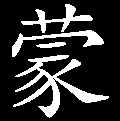
\includegraphics[width=3mm]{../Images/00006}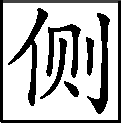
\includegraphics[width=3mm]{../Images/00011}\footnotesize \kaishu 教导之法、慈悲之心尽矣,无奈迷{(徒)}{[}途{]}不悟何!}好容易盼到早晨,只见一个老婆子先将东门开了,进去又叫西门。贾瑞瞅他背着脸,一溜烟抱着肩跑了出来,幸而天气尚早,人都未起,从后门一径跑回家去。

原来贾瑞父母早亡,只有他祖父代儒教养。那代儒素日教训最严,{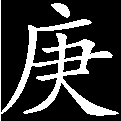
\includegraphics[width=3mm]{../Images/00004}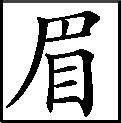
\includegraphics[width=3mm]{../Images/00010}\footnotesize \kaishu 教训最严,奈其心何!一叹。}不许贾瑞多走一步,生怕他在外吃酒赌钱,有误学业。今忽见他一夜不归,只料定他在外非饮即赌,嫖娼宿妓,{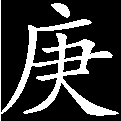
\includegraphics[width=3mm]{../Images/00004}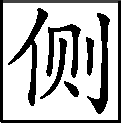
\includegraphics[width=3mm]{../Images/00011}\footnotesize \kaishu 展转灵活,一人不放,一笔不肖。}那里想到这段公案,{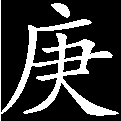
\includegraphics[width=3mm]{../Images/00004}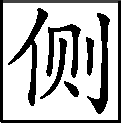
\includegraphics[width=3mm]{../Images/00011}\footnotesize \kaishu 世人万万想不到,况老学究乎!}因此气了一夜。贾瑞也捻着一把汗,少不得回来撒谎,只说:``往舅舅家去了,天黑了,留我住了一夜。''代儒道:``自来出门,非禀我不敢擅出,如何昨日私自去了?据此亦该打,何况是撒谎!''{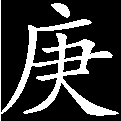
\includegraphics[width=3mm]{../Images/00004}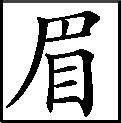
\includegraphics[width=3mm]{../Images/00010}\footnotesize \kaishu 处处点父母痴心、子孙不肖。此书系自愧而成。}因此,发狠到底打了三四十板,不许吃饭,令他跪在院内读文章,定要补出十天工课来方罢。贾瑞直冻了一夜,今又遭了苦打,且饿着肚子跪在风地里念文章,{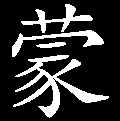
\includegraphics[width=3mm]{../Images/00006}\includegraphics[width=3mm]{../Images/00011}\footnotesize \kaishu 教令何尝不好,孽种故此不同。}其苦万状。{\includegraphics[width=3mm]{../Images/00003}\includegraphics[width=3mm]{../Images/00012}\footnotesize \kaishu 祸福无门,唯人自招。}

此时贾瑞前心犹是未改,{\includegraphics[width=3mm]{../Images/00004}\includegraphics[width=3mm]{../Images/00011}\footnotesize \kaishu 四字是寻死之根。 \includegraphics[width=3mm]{../Images/00004}\includegraphics[width=3mm]{../Images/00010}\footnotesize \kaishu 苦海无边,回头是岸。若个能回头也?叹叹!壬午春。畸笏。}再想不到是凤姐捉弄他。过后两日,得了空,便仍来找凤姐。凤姐故意抱怨他失信,贾瑞急的赌身发誓。凤姐因见他自投罗网,{\includegraphics[width=3mm]{../Images/00004}\includegraphics[width=3mm]{../Images/00011}\footnotesize \kaishu 可谓因人而使。}少不得再寻别计令他知改,{\includegraphics[width=3mm]{../Images/00004}\includegraphics[width=3mm]{../Images/00011}\footnotesize \kaishu 四字是作者明阿凤身份,勿得轻轻看过。}故又约他道:``今日晚上,你别在那里了。你在我这房后小过道子里那间空屋里等我,可别冒撞了。''{\includegraphics[width=3mm]{../Images/00003}\includegraphics[width=3mm]{../Images/00012}\footnotesize \kaishu 伏的妙!}贾瑞道:``果真?''凤姐道:``谁可哄你,你不信就别来。''{{\includegraphics[width=3mm]{../Images/00004}\includegraphics[width=3mm]{../Images/00011}\footnotesize \kaishu 紧一句。 }\includegraphics[width=3mm]{../Images/00006}\includegraphics[width=3mm]{../Images/00011}\footnotesize \kaishu 大士心肠。}贾瑞道:``来,来,来。死也要来!''{\includegraphics[width=3mm]{../Images/00003}\includegraphics[width=3mm]{../Images/00012}\footnotesize \kaishu 不差。}凤姐道:``这会子你先去罢。''贾瑞料定晚间必妥,{\includegraphics[width=3mm]{../Images/00004}\includegraphics[width=3mm]{../Images/00011}\footnotesize \kaishu 未必。}此时先去了。凤姐在这里便点兵派将,{{\includegraphics[width=3mm]{../Images/00004}\includegraphics[width=3mm]{../Images/00011}\footnotesize \kaishu 四字用得新,必有新文字好看。 }\includegraphics[width=3mm]{../Images/00006}\includegraphics[width=3mm]{../Images/00011}\footnotesize \kaishu {(剩)}{[}新{]}文,最妙!}设下圈套。

那贾瑞只盼不到夜上,偏生家里有亲戚又来了,{\includegraphics[width=3mm]{../Images/00003}\includegraphics[width=3mm]{../Images/00012}\footnotesize \kaishu 专能忙中写闲,狡猾之甚!}直等吃了晚饭才去,那天已有掌灯时候。又等他祖父安歇了,方溜进荣府,直往那夹道中屋子里来等着,热锅上的蚂蚁一般,{\includegraphics[width=3mm]{../Images/00006}\includegraphics[width=3mm]{../Images/00011}\footnotesize \kaishu 有心人记着,其实苦恼。}只是干转。左等不见人影,右闻也没声音,心下自思:``别是又不来了,又冻我一夜不成?''{\includegraphics[width=3mm]{../Images/00006}\includegraphics[width=3mm]{../Images/00011}\footnotesize \kaishu 似醒非醒语。}正自胡猜,只见黑魆魆的来了一个人,{\includegraphics[width=3mm]{../Images/00004}\includegraphics[width=3mm]{../Images/00011}\footnotesize \kaishu 真到了。}贾瑞便意定是凤姐,不管皂白,饿虎一般,等那人刚至门前,便如猫儿捕鼠的一般,抱住叫道:``亲嫂子,等死我了。''说着,抱到屋里炕上就亲嘴扯裤子,满口里``亲娘''``亲爹''的乱叫起来。{\includegraphics[width=3mm]{../Images/00006}\includegraphics[width=3mm]{../Images/00011}\footnotesize \kaishu 丑态可笑。}那人只不做声,{\includegraphics[width=3mm]{../Images/00004}\includegraphics[width=3mm]{../Images/00011}\footnotesize \kaishu 好极!}贾瑞拉了自己裤子,硬帮帮的就想顶入。{\includegraphics[width=3mm]{../Images/00004}\includegraphics[width=3mm]{../Images/00011}\footnotesize \kaishu 将到矣。}忽然灯光一闪,只见贾蔷举着个捻子照道:``谁在屋里?''只见炕上那人笑道:``瑞大叔要臊我呢。''贾瑞一见,却是贾蓉,{\includegraphics[width=3mm]{../Images/00003}\includegraphics[width=3mm]{../Images/00012}\footnotesize \kaishu 奇绝!}真臊的无地可入,{\includegraphics[width=3mm]{../Images/00004}\includegraphics[width=3mm]{../Images/00011}\footnotesize \kaishu 亦未必真。}不知要怎么样才好,回身就要跑,被贾蔷一把揪住道:``别走!如今琏二婶已经告到太太跟前,{\includegraphics[width=3mm]{../Images/00004}\includegraphics[width=3mm]{../Images/00011}\footnotesize \kaishu 好题目。}说你无故调戏他。{\includegraphics[width=3mm]{../Images/00004}\includegraphics[width=3mm]{../Images/00010}\footnotesize \kaishu 调戏还有故?一笑。}他暂用了个脱身计,哄你在这边等着,太太气死过去,{\includegraphics[width=3mm]{../Images/00004}\includegraphics[width=3mm]{../Images/00011}\footnotesize \kaishu 好大题目。}因此叫我来拿你。刚才你又拦住他,没的说,跟我去见太太!''

贾瑞听了,魂不附体,只说:``好侄儿,只说没有见我,明日我重重的谢你。''贾蔷道:``你若谢我,放你不值什么,只不知你谢我多少?况且口说无凭,写一文契来。''贾瑞道:``这如何落纸呢?''{\includegraphics[width=3mm]{../Images/00004}\includegraphics[width=3mm]{../Images/00011}\footnotesize \kaishu 也知写不得。一叹!}贾蔷道:``这也不妨,写一个赌钱输了外人账目,借头家银若干两便罢。''贾瑞道:``这也容易。只是此时无纸笔。''贾蔷道:``这也容易。''说罢,翻身出来,纸笔现成,{\includegraphics[width=3mm]{../Images/00004}\includegraphics[width=3mm]{../Images/00011}\footnotesize \kaishu 二字妙!}拿来命贾瑞写。他两个作好作歹,只写了五十两银,然后画了押,贾蔷收起来。然后撕罗贾蓉。{\includegraphics[width=3mm]{../Images/00006}\includegraphics[width=3mm]{../Images/00011}\footnotesize \kaishu 可怜至此!好事者当自度。}贾蓉先咬定牙不依,只说:``明日告诉族中的人评评理。''贾瑞急的至于叩头。贾蔷做好做歹的,{\includegraphics[width=3mm]{../Images/00006}\includegraphics[width=3mm]{../Images/00011}\footnotesize \kaishu 此是加一倍法。}也写了一张五十两欠契才罢。贾蔷又道:``如今要放你,我就担着不是。{\includegraphics[width=3mm]{../Images/00003}\includegraphics[width=3mm]{../Images/00012}\footnotesize \kaishu 又生波澜。}老太太那边的门早已关了,老爷正在厅上看南京的东西,那一条路定难过去,如今只好走后门。若这一走,倘或遇见了人,连我也完了。等我们先去哨探哨探,再来领你。这屋你还藏不得,少时就来堆东西。等我寻个地方。''说毕,拉着贾瑞,仍熄了灯,{\includegraphics[width=3mm]{../Images/00003}\includegraphics[width=3mm]{../Images/00012}\footnotesize \kaishu 细。}出至院外,摸着大台矶底下,说道:``这窝儿里好,你只蹲着,别哼一声,等我们来再动。''{\includegraphics[width=3mm]{../Images/00004}\includegraphics[width=3mm]{../Images/00011}\footnotesize \kaishu 未必如此收场。}说毕,二人去了。

贾瑞此时身不由己,只得蹲在那里。心下正盘算,只听头顶上一声响,哗拉拉一净桶尿粪从上面直泼下来,可巧浇了他一头一身,贾瑞撑不住``嗳哟''了一声,忙又掩住口,{\includegraphics[width=3mm]{../Images/00003}\includegraphics[width=3mm]{../Images/00012}\footnotesize \kaishu 更奇。}不敢声张,满头满脸浑身皆是尿屎,冰冷打战。{{\includegraphics[width=3mm]{../Images/00004}\includegraphics[width=3mm]{../Images/00011}\footnotesize \kaishu 余料必{[}有{]}新奇解恨文字收场,方是《石头记》笔力。 \includegraphics[width=3mm]{../Images/00004}\includegraphics[width=3mm]{../Images/00010}\footnotesize \kaishu 瑞奴实当如是报之。◇此一节可入《西厢记》批评内十大快中。畸笏。 }\includegraphics[width=3mm]{../Images/00006}\includegraphics[width=3mm]{../Images/00011}\footnotesize \kaishu 这也未必不是预为埋伏者。总是慈悲设教,遇难教者,不得不现三头六臂,并吃人心、喝人血之相,以警戒之耳。}只见贾蔷跑来叫:``快走,快走!''贾瑞如得了命,三步两步从后门跑到家里,天已三更,只得叫门。开门人见他这般光景,问是怎的。少不得撒谎说:``黑了,失脚掉在茅厕里了。''一面到自己房中更衣洗濯,心下方想到是凤姐顽他,因此发一回恨;再想想凤姐的模样儿,{\includegraphics[width=3mm]{../Images/00004}\includegraphics[width=3mm]{../Images/00011}\footnotesize \kaishu 欲根未断。}又恨不得一时搂在怀,一夜竟不曾合眼。

自此满心想凤姐,{{\includegraphics[width=3mm]{../Images/00004}\includegraphics[width=3mm]{../Images/00010}\footnotesize \kaishu 此刻还不回头,真自寻死路矣。 }\includegraphics[width=3mm]{../Images/00006}\includegraphics[width=3mm]{../Images/00011}\footnotesize \kaishu 孙行者非有紧箍儿,虽老君之炉、五行之山,何尝屈其一二?}只不敢往荣府去了。贾蓉两个常常的来索银子,他又怕祖父知道,正是相思尚且难禁,更又添了债务;日间工课又紧,他二十来岁之人,尚未娶亲,迩来想着凤姐,未免有那指头告了消乏等事;更兼两回冻恼奔波,{\includegraphics[width=3mm]{../Images/00003}\includegraphics[width=3mm]{../Images/00012}\footnotesize \kaishu 写得历历病源,如何不死?}因此三五下里夹攻,{\includegraphics[width=3mm]{../Images/00004}\includegraphics[width=3mm]{../Images/00011}\footnotesize \kaishu 所谓步步紧。}不觉就得了一病:心内发膨胀,口内无滋味,脚下如绵,眼中似醋,黑夜作烧,白昼常倦,下溺连精,嗽痰带血。诸如此症,不上一年,都添全了。{\includegraphics[width=3mm]{../Images/00004}\includegraphics[width=3mm]{../Images/00011}\footnotesize \kaishu 简捷之至!}于是不能支持,一头睡倒,合上眼还只梦魂颠倒,满口乱说胡话,惊怖异常。百般请医治疗,诸如肉桂、附子、鳖甲、麦冬、玉竹等药,吃了有几十斤下去,也不见个动静。{\includegraphics[width=3mm]{../Images/00003}\includegraphics[width=3mm]{../Images/00012}\footnotesize \kaishu 说得有趣。}

倏又腊尽春回,这病更又沉重。代儒也着了忙,各处请医疗治,皆不见效。因后来吃``独参汤'',代儒如何有这力量,只得往荣府来寻。王夫人命凤姐秤二两给他,{\includegraphics[width=3mm]{../Images/00003}\includegraphics[width=3mm]{../Images/00012}\footnotesize \kaishu 王夫人之慈若是。}凤姐回说:``前儿新近都替老太太配了药,那整的太太又说留着送杨提督的太太配药,偏生昨儿我已送了去了。''王夫人道:``就是咱们这边没了,你打发个人往你婆婆那边问问,或是你珍大哥哥那府里再寻些来,凑着给人家。吃好了,救人一命,也是你的好处。''{\includegraphics[width=3mm]{../Images/00003}\includegraphics[width=3mm]{../Images/00012}\footnotesize \kaishu 夹写王夫人。}凤姐听了,也不遣人去寻,只得将些渣末泡须凑了几钱,命人送去,只说:{\includegraphics[width=3mm]{../Images/00006}\includegraphics[width=3mm]{../Images/00011}\footnotesize \kaishu ``只说''。}``太太送来的,再也没了。''然后回王夫人说:``都寻了来,共凑了有二两多送去。''{\includegraphics[width=3mm]{../Images/00003}\includegraphics[width=3mm]{../Images/00012}\footnotesize \kaishu 然便有二两独参汤,贾瑞固亦不能好,又岂能望好,但凤姐之毒何如是耶?终是瑞之自失。}

那贾瑞此时要命心胜,无药不吃,只是白花钱,不见效。忽然这日有个跛足道人{\includegraphics[width=3mm]{../Images/00003}\includegraphics[width=3mm]{../Images/00012}\footnotesize \kaishu 自甄士隐随君一去,别来无恙否?}来化斋,口称专治冤业之症。贾瑞偏生在内就听见了,直着声叫喊{\includegraphics[width=3mm]{../Images/00003}\includegraphics[width=3mm]{../Images/00012}\footnotesize \kaishu 如闻其声,吾不忍听也。}说:``快请进那位菩萨来救我!''一面叫,一面在枕上叩首。{\includegraphics[width=3mm]{../Images/00003}\includegraphics[width=3mm]{../Images/00012}\footnotesize \kaishu 如见其形,吾不忍看也。}众人只得带了那道士进来。贾瑞一把拉住,连叫:``菩萨救我!''{\includegraphics[width=3mm]{../Images/00003}\includegraphics[width=3mm]{../Images/00012}\footnotesize \kaishu 人之将死,其言也哀,作者如何下笔?}那道士叹道:``你这病非药可医!我有个宝贝与你,你天天看时,此命可保矣。''说毕,从褡裢中{\includegraphics[width=3mm]{../Images/00003}\includegraphics[width=3mm]{../Images/00012}\footnotesize \kaishu 妙极!此褡裢犹是士隐所抢背者乎?}取出一面镜子来{\includegraphics[width=3mm]{../Images/00003}\includegraphics[width=3mm]{../Images/00012}\footnotesize \kaishu 凡看书者从此细心体贴,方许你看,否则此书哭矣。}------两面皆可照人,{\includegraphics[width=3mm]{../Images/00003}\includegraphics[width=3mm]{../Images/00012}\footnotesize \kaishu 此书表里皆有喻也。}镜把上面錾着``风月宝鉴''四字{\includegraphics[width=3mm]{../Images/00003}\includegraphics[width=3mm]{../Images/00012}\footnotesize \kaishu 明点。}------递与贾瑞道:``这物出自太虚幻境空灵殿上,警幻仙子所制,{\includegraphics[width=3mm]{../Images/00003}\includegraphics[width=3mm]{../Images/00012}\footnotesize \kaishu 言此书原系空虚幻设。 {\includegraphics[width=3mm]{../Images/00004}\includegraphics[width=3mm]{../Images/00010}\footnotesize \kaishu 与``红楼梦''呼应。}}专治邪思妄动之症,{\includegraphics[width=3mm]{../Images/00003}\includegraphics[width=3mm]{../Images/00012}\footnotesize \kaishu 毕真。}有济世保生之功。{\includegraphics[width=3mm]{../Images/00003}\includegraphics[width=3mm]{../Images/00012}\footnotesize \kaishu 毕真。}所以带他到世上,单与那些聪明俊杰、风雅王孙等看照。{\includegraphics[width=3mm]{../Images/00003}\includegraphics[width=3mm]{../Images/00012}\footnotesize \kaishu 所谓无能纨绔是也。}千万不可照正面,{\includegraphics[width=3mm]{../Images/00003}\includegraphics[width=3mm]{../Images/00012}\footnotesize \kaishu 观者记之,不要看这书正面,方是会看。 {\includegraphics[width=3mm]{../Images/00004}\includegraphics[width=3mm]{../Images/00011}\footnotesize \kaishu 谁人识得此句!}}只照他的背面,{\includegraphics[width=3mm]{../Images/00003}\includegraphics[width=3mm]{../Images/00012}\footnotesize \kaishu 记之。}要紧,要紧!三日后吾来收取,管叫你好了。''说毕,佯常而去,众人苦留不住。

贾瑞收了镜子,想道:``这道士倒有些意思,我何不照一照试试。''想毕,拿起``风月鉴''来,向反面一照,只见一个骷髅立在里面,{\includegraphics[width=3mm]{../Images/00003}\includegraphics[width=3mm]{../Images/00012}\footnotesize \kaishu 所谓``好知青冢骷髅骨,就是红楼掩面人''是也。作者好苦心思。}唬得贾瑞连忙掩了,骂:``道士混账,如何吓我!我倒再照照正面是什么。''想着,又将正面一照,只见凤姐站在里面招手{\includegraphics[width=3mm]{../Images/00004}\includegraphics[width=3mm]{../Images/00011}\footnotesize \kaishu 可怕是``招手''二字。}叫他。{\includegraphics[width=3mm]{../Images/00003}\includegraphics[width=3mm]{../Images/00012}\footnotesize \kaishu 奇绝!}贾瑞心中一喜,荡悠悠的觉得进了镜子,{\includegraphics[width=3mm]{../Images/00003}\includegraphics[width=3mm]{../Images/00012}\footnotesize \kaishu 写得奇峭,真好笔墨。}与凤姐云雨一番,凤姐仍送他出来。到了床上,``嗳哟''了一声,一睁眼,镜子从手里掉过来,仍是反面立着一个骷髅。贾瑞自觉汗津津的,底下已遗了一滩精。{\includegraphics[width=3mm]{../Images/00006}\includegraphics[width=3mm]{../Images/00011}\footnotesize \kaishu 此一句力如龙象,意谓:正面你方才已自领略了,你也当思想反面才是。}心中到底不足,又翻过正面来,只见凤姐还招手叫他,他又进去。如此三四次。到了这次,刚要出镜子来,只见两个人走来,拿铁锁把他套住,拉了就走。{\includegraphics[width=3mm]{../Images/00003}\includegraphics[width=3mm]{../Images/00012}\footnotesize \kaishu 所谓醉生梦死也。}贾瑞叫道:``让我拿了镜子再走!''{\includegraphics[width=3mm]{../Images/00003}\includegraphics[width=3mm]{../Images/00012}\footnotesize \kaishu 可怜!大众齐来看此。 \includegraphics[width=3mm]{../Images/00006}\includegraphics[width=3mm]{../Images/00011}\footnotesize \kaishu 这是作书者之立意,要写情种,故于此试一深写之。在贾瑞则是求仁而得仁,未尝不含笑九泉,虽死后亦不解脱者,悲矣!}------只说了这句,就再不能说话了。

旁边伏侍贾瑞的众人,只见他先还拿着镜子照,落下来,仍睁开眼拾在手内,末后镜子落下来便不动了。众人上来看看,已没了气,身子底下冰凉渍湿一大滩精,这才忙着穿衣抬床。代儒夫妇哭的死去活来,大骂道士,``是何妖镜!{\includegraphics[width=3mm]{../Images/00003}\includegraphics[width=3mm]{../Images/00012}\footnotesize \kaishu 此书不免腐儒一谤。}若不早毁此物,{\includegraphics[width=3mm]{../Images/00003}\includegraphics[width=3mm]{../Images/00012}\footnotesize \kaishu 凡野史俱可毁,独此书不可毁。}遗害于世不小。''{\includegraphics[width=3mm]{../Images/00003}\includegraphics[width=3mm]{../Images/00012}\footnotesize \kaishu 腐儒。}遂命架火来烧,只听镜内哭道:``谁叫你们瞧正面了!你们自己以假为真,何苦来烧我?''{\includegraphics[width=3mm]{../Images/00003}\includegraphics[width=3mm]{../Images/00012}\footnotesize \kaishu 观者记之。}正哭着,只见那跛足道人从外跑来,喊道:``谁毁`风月鉴',吾来救也!''说着,直入中堂,抢入手内,飘然去了。

当下,代儒料理丧事,各处去报丧。三日起经,七日发引,寄灵于铁槛寺,{\includegraphics[width=3mm]{../Images/00003}\includegraphics[width=3mm]{../Images/00012}\footnotesize \kaishu 所谓``铁门限''是也。先安一开路之人,以备秦氏仙柩有方也。}日后带回原籍。当下贾家众人齐来吊问,荣府贾赦赠银二十两,贾政亦是二十两,宁国府贾珍亦有二十两,别者族中人贫富不等,或三两五两,不可胜数。另有各同窗家分资,也凑了二三十两。代儒家道虽然淡薄,倒也丰丰富富完了此事。

谁知这年冬底\href{../Text/part0016_split_000.html\#lnkback_1_a}{\textsuperscript{①}},林如海的书信寄来,却为身染重疾,写书特来接林黛玉回去。{\includegraphics[width=3mm]{../Images/00006}\includegraphics[width=3mm]{../Images/00011}\footnotesize \kaishu 须要林黛玉长住,偏要暂离。}贾母听了,未免又加忧闷,只得忙忙的打点黛玉起身。宝玉大不自在,争奈父女之情,也不好拦劝。于是贾母定要贾琏送他去,仍叫带回来。一应土仪盘缠,不消烦说,自然要妥贴。作速择了日期,贾琏与林黛玉辞别了贾母等,带领仆从,登舟往扬州去了。要知端的,且听下回分解。

{{\includegraphics[width=3mm]{../Images/00004}  \kaishu 此回忽遣黛玉去者,正为下回可儿之文也。若不遣去,只写可儿、阿凤等人,却置黛玉于荣府,成何文哉?故必遣去,方好放笔写秦,方不脱节。况黛玉乃书中正人,秦为陪客,岂因陪而失正耶?后大观园方是宝玉、宝钗、黛玉等正经文字,前皆系陪衬之文也。}}

{\includegraphics[width=3mm]{../Images/00005}  \kaishu  总评:儒家正心,道者炼心,释辈戒心。可见此心无有不到,无不能入者,独畏其入于邪而不反,故用心炼戒以缚之。请看贾瑞一起念,及至于死,专诚不二,虽经两次警教,毫无反悔,可谓痴子,可谓愚情。相乃可思,不能相而独欲思,岂逃倾颓?作者以此作一新样情种,以助解者生笑,以为痴者设一棒喝耳!}

{\href{../Text/part0016_split_000.html\#navto_1_a}{①}按:``冬底'',各本均同,但与上下文时间不衔接。吴克歧假托古本作``八月底'',林冠夫理校为``五月底'',可参考。}
